\documentclass[12pt]{article}
\usepackage[T1]{fontenc}
\usepackage{polski}
\usepackage[utf8]{inputenc}
\newcommand{\BibTeX}{{\sc Bib}\TeX} 
\usepackage{graphicx}
\usepackage{amsfonts}

\setlength{\textheight}{21cm}

\title{{\bf Zadanie nr 1 -  Sieć Kohonena do kompresji obrazów}\linebreak
Inteligentne przetwarzanie danych}
\author{Tomasz Stachura, 233264 \and Łukasz Rogoziński, 233261}
\date{16.05.2020}

\begin{document}
\clearpage\maketitle
\thispagestyle{empty}
\newpage
\setcounter{page}{1}
\section{Cel zadania}
Celem zadania była implementacja sieć neuronowej Kohonena do kompresji obrazu

\section{Wstęp teoretyczny}

\subsection{Algorytm Kohonena}
 Sieć Kohonena to samo-organizująca się mapa wykorzystująca  algorytm uczenia się bez nadzoru, używanym do zmniejszania wymiarów danych i grupowania danych. Jej struktura składa się z jednowarstwowej liniowej dwuwymiarowej siatki neuronów. Wszystkie węzły na tej siatce są podłączone tylko i wyłącznie bezpośrednio do wektora wejściowego. Oznacza to, że węzły nie znają wartości swoich sąsiadów i jedynie aktualizują wagę swoich połączeń w zależności od danych wejściowych. Sama siatka jest mapą, która organizuje się przy każdej iteracji w zależności od danych wejściowych. Dobór wag neuronów jest realizowany według wzoru (1).
\begin{equation}
    w_i_j(t+1)= w_i_j(t)+\alpha_i(t)\beta_i_j[x(t)-w_i_j(t)]
\end{equation}
 Zaktualizowana waga powinna uwzględniać fakt, że efekt uczenia się jest prawie żaden na krańcach sąsiedztwa, ponieważ ilość uczenia się powinna maleć wraz z odległością. Dlatego wagi modyfikowane są z wykorzystaniem gaussowskiej funkcji sąsiedztwa βij (t), którą można zapisać:
\begin{equation}
\beta_i_j(t)=\exp\left(-\frac{d^2(i,j)}{2\sigma^2(t)}\right)
\end{equation}
gdzie $d(i,j)$ jest odległością Euklidesową pomiędzy zwycięzcą $(j)$, a i-tym
neuronem z sąsiedztwa. Odległość euklidesowa między wektorem ciężaru każdego węzła a bieżącą instancją wejściową jest obliczana na podstawie wzoru Pitagorasa.
\begin{equation}
d = min( || \overrightarrow{x} - \overrightarrow{w_i_j} || ) =min \left(\sqrt{\sum_{t=0}^{n}[\overrightarrow{x}(t) - \overrightarrow{w_i_j}(t)]^{2}}\right)
\end{equation}
Promień i szybkość uczenia się są z czasem podobnie i wykładniczo zanikają. Gdzie $ \sigma(t) $ jest promieniem funkcji sąsiedztwa, a $ \alpha(t) $   to szybkość uczenia się, która maleje z czasem w przedziale [0,1], aby zapewnić zbieżność sieci.
\begin{equation}
\sigma (t)=\sigma_0 \cdot \exp\left(\frac{-t}{\lambda }\right)
\end{equation}
\begin{equation}
\alpha  (t)=\alpha_0 \cdot \exp\left(\frac{-t}{\lambda }\right)
\end{equation}
Algorytm ten można wyrazić w kategoriach modelu enkodera-dekodera stosowanego do kwantyzacji wektorów. Podczas kodowania dowiadujemy się o Best Matching Unit (BMU) lub neuronie zwycięzcy. W sieci neuronów każdemu neuronowi przypisane jest słowo kodowe. Słowo kodowe odpowiadające zwycięskiemu neuronowi jest przekazywane do dekodera. Podczas dekodowania musimy znaleźć wektor rekonstrukcji z otrzymanego słowa kodowego. Ten wektor rekonstrukcji jest wektorem wagi odpowiadającym zwycięskiemu neuronowi.
\section{Eksperymenty i wyniki}

Przeprowadziliśmy 4 eksperymenty, dzięki którym poznaliśmy jak odpowiednie współczynniki wpływają na jakość skompresowanego obrazu, poziom jego kompresji oraz czas potrzebny do jego skompresowania. W eksperymentach poddany był obraz Lena.jpg, który możemy zobaczyć na poniższej grafice.

\begin{figure}[h!]
 \centering
 
 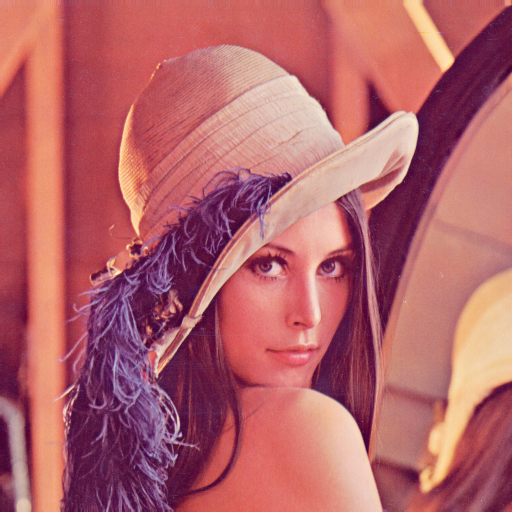
\includegraphics[width=10cm]{Lenna.png}
 \vspace{-0.3cm}
 \caption{Obraz Lena poddawany kompresji}
 \vspace*{\floatsep}


\end{figure}
\clearpage


%%%%%%%%%%%%%%%%%%%%%%%%%%%%%%%%%%%%%%%%%%%%%%%%%%%%%%%%%%%%%%%%%%%%%%%%%%%%%%%%%%%%%%%%%%%%%%%%%%%%%%%%%%%%%%%%%
% PODROZDZIA£ PT. EKSPERYMENT NR 1 
%%%%%%%%%%%%%%%%%%%%%%%%%%%%%%%%%%%%%%%%%%%%%%%%%%%%%%%%%%%%%%%%%%%%%%%%%%%%%%%%%%%%%%%%%%%%%%%%%%%%%%%%%%%%%%%%%
\newpage
\subsection{Eksperyment nr 1}

Eksperyment nr 1 polegał sprawdzeniu jaki efekt przyniesie kompresja obrazu ze względu na różną ilość neuronów w warstwie wyjściowej. Zrealizowano 3 przypadki testowe odpowiednio dla wartości przedstawionych w Tab.
\ref{dane eksperymentalne doświadczenia 1}. \\
\begin{table}[h!]
 \caption{Dane eksperymentalne nr 1}
 \centering
 \vspace{0.2cm}
 \begin{tabular}{c c}
  \hline\hline\\[-0.4cm]
  \textbf{Przypadek} & \textbf{Ilość neuronów} \\[0.1cm]
  \textbf{1} & 5  \\
  \textbf{2} & 30  \\
  \textbf{3} & 300  \\ [0.1cm]
  \hline
 \end{tabular}
 \label{dane eksperymentalne doświadczenia 1}
\end{table} \\
Dla każdego z wyżej wymienionych przypadków ustawiliśmy następujące wartości: \\
\begin{table}[h!]
 \caption{Dodatkowe dane do eksperymentu nr 1}
 \centering
 \vspace{0.2cm}
 \begin{tabular}{c c c}
  \hline\hline\\[-0.4cm]
  \textbf{Wielkość ramki} & \textbf{Krok uczenia} & \textbf{Ilość ramek treningowych} \\[0.1cm]
  4x4 & 0.2 & 5000  \\ [0.1cm]
  \hline
 \end{tabular}
 \label{dodatkowe dane do eksperymentu nr 1}
\end{table} \\

\subsubsection{Rezultat}

Wynik powyższego doświadczenia przedstawiony został w Tab.
\ref{wynik eksperymentu 1}.

\begin{table}[h!]
 \caption{Wynik eksperymentu nr 1}
 \centering
 \vspace{0.2cm}
 \begin{tabular}{c c c c}
  \hline\hline\\[-0.4cm]
  \textbf{Przypadek} & \textbf{MSR} & \textbf{PSNR} & \textbf{Compression Ratio} \\[0.1cm]
  \textbf{1} & 350.88 & 22.68 & 25.68  \\
  \textbf{2} & 125.72 & 27.14 & 8.27  \\
  \textbf{3} & 106.72 & 27.85 & 4.96  \\ [0.1cm]
  \hline
 \end{tabular}
 \label{wynik eksperymentu 1}
\end{table}

Z otrzymanych wyników można wywnioskować, iż ilość neuronów wpływa na stopień kompresji obrazka oraz na jego jakość. Im więcej neuronów, tym dokładniejszy obrazek zostanie wygenerowany, jednocześnie stopień kompresji znacząco się zmniejsza. Widoczna jest również wyraźna różnica w kolorze, im więcej neuronów, tym lepsze odwzorowanie kolorów. Poniżej możemy porównać obrazek z przypadku nr 1 oraz przypadku nr 3.

\begin{figure}[h!]
 \centering
 
 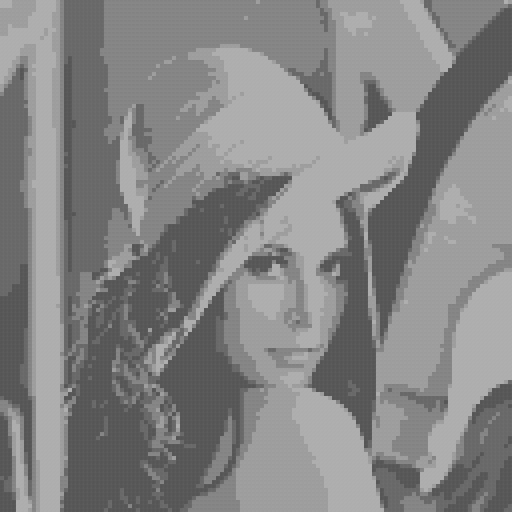
\includegraphics[width=10cm]{CB_neurons=5_block_size=4x4.png}
 \vspace{-0.3cm}
 \caption{Skompresowany obraz otrzymany z przypadku 1}
 \vspace*{\floatsep}

 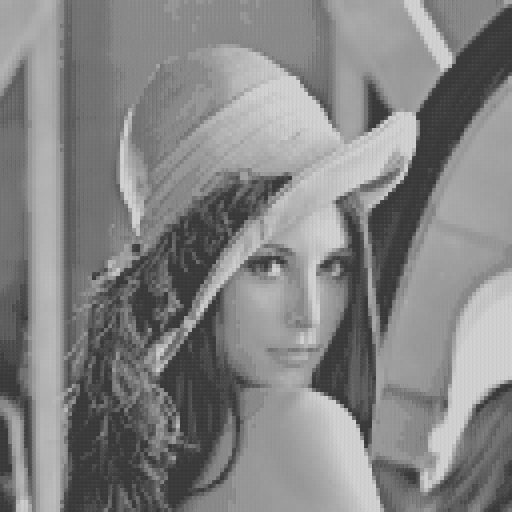
\includegraphics[width=10cm]{CB_neurons=300_block_size=4x4.png}
 \vspace{-0.3cm}
 \caption{Skompresowany obraz otrzymany z przypadku 3}

\end{figure}



%%%%%%%%%%%%%%%%%%%%%%%%%%%%%%%%%%%%%%%%%%%%%%%%%%%%%%%%%%%%%%%%%%%%%%%%%%%%%%%%%%%%%%%%%%%%%%%%%%%%%%%%%%%%%%%%%
% PODROZDZIAł PT. EKSPERYMENT NR 2 
%%%%%%%%%%%%%%%%%%%%%%%%%%%%%%%%%%%%%%%%%%%%%%%%%%%%%%%%%%%%%%%%%%%%%%%%%%%%%%%%%%%%%%%%%%%%%%%%%%%%%%%%%%%%%%%%%
\clearpage
\subsection{Eksperyment nr 2}

Eksperyment nr 2 polegał sprawdzeniu jak zostanie skompresowany obraz zmieniając wielkość ramek, na jakie zostaje podzielony obraz wejściowy. Zrealizowano 3 przypadki testowe odpowiednio dla wartości przedstawionych w Tab.
\ref{dane eksperymentalne doświadczenia 2}. \\
\begin{table}[h!]
 \caption{Dane eksperymentalne nr 2}
 \centering
 \vspace{0.2cm}
 \begin{tabular}{c c}
  \hline\hline\\[-0.4cm]
  \textbf{Przypadek} & \textbf{Wielkość ramki} \\[0.1cm]
  \textbf{1} & 4x4  \\
  \textbf{2} & 8x8  \\
  \textbf{3} & 16x16  \\ [0.1cm]
  \hline
 \end{tabular}
 \label{dane eksperymentalne doświadczenia 2}
\end{table} \\

Dla każdego z wyżej wymienionych przypadków ustawiliśmy następujące wartości: \\
\begin{table}[h!]
 \caption{Dodatkowe dane do eksperymentu nr 2}
 \centering
 \vspace{0.2cm}
 \begin{tabular}{c c c}
  \hline\hline\\[-0.4cm]
  \textbf{Ilość neuronów} & \textbf{Krok uczenia} & \textbf{Ilość ramek treningowych} \\[0.1cm]
  40 & 0.2 & 5000  \\ [0.1cm]
  \hline
 \end{tabular}
 \label{dodatkowe dane do eksperymentu nr 2}
\end{table} \\

\newpage
\subsubsection{Rezultat}

Wynik powyższego doświadczenia przedstawiony został w Tab.
\ref{wynik eksperymentu 2}.

\begin{table}[h!]
 \caption{Wynik eksperymentu nr 2}
 \centering
 \vspace{0.2cm}
 \begin{tabular}{c c c c}
  \hline\hline\\[-0.4cm]
  \textbf{Przypadek} & \textbf{MSR} & \textbf{PSNR} & \textbf{Compression Ratio} \\[0.1cm]
  \textbf{1} & 119.76 & 27.35 & 7.35  \\
  \textbf{2} & 164.93 & 25.96 & 10.89  \\
  \textbf{3} & 299.90 & 23.36 & 11.93  \\ [0.1cm]
  \hline
 \end{tabular}
 \label{wynik eksperymentu 2}
\end{table}

Otrzymane wyniki mówią nam jasno, iż wielkość ramki ma duże znaczenie przy kompresji obrazu. Im większą ramkę zdefiniowaliśmy, tym obraz był bardziej skompresowany, aczkolwiek tracił znacznie na jakości i szczegółowości. Możemy to dobrze zaobserwować na poniższych obrazach przedstawiających kolejno 2 oraz 3 przypadek testowy. Zdecydowaliśmy się pokazać wyżej wymienione przypadki ponieważ przypadek nr 1 jest pod względem jakości bardzo zbliżony do przypadku 3 z eksperymentu 1.

\begin{figure}[h!]
 \centering
 
 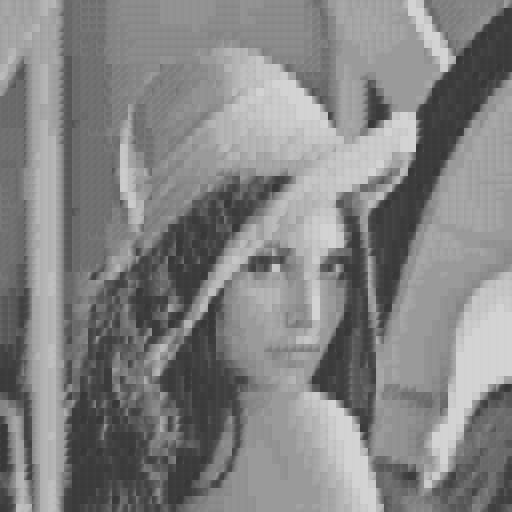
\includegraphics[width=10cm]{CB_neurons=40_block_size=8x8.png}
 \vspace{-0.3cm}
 \caption{Skompresowany obraz otrzymany z przypadku 2}
 \vspace*{\floatsep}

 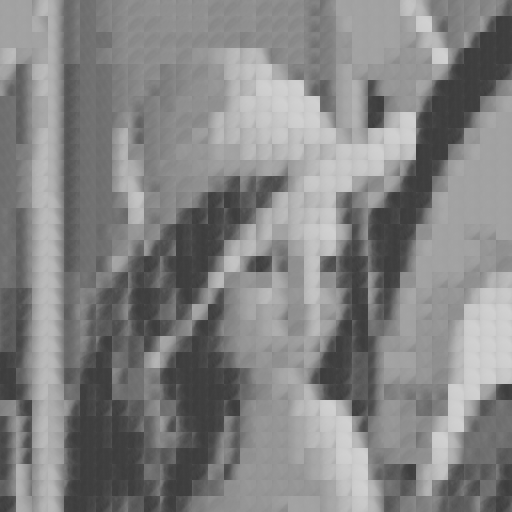
\includegraphics[width=10cm]{CB_neurons=40_block_size=16x16.png}
 \vspace{-0.3cm}
 \caption{Skompresowany obraz otrzymany z przypadku 3}

\end{figure}
\clearpage

%%%%%%%%%%%%%%%%%%%%%%%%%%%%%%%%%%%%%%%%%%%%%%%%%%%%%%%%%%%%%%%%%%%%%%%%%%%%%%%%%%%%%%%%%%%%%%%%%%%%%%%%%%%%%%%%%
% PODROZDZIA£ PT. EKSPERYMENT NR 3
%%%%%%%%%%%%%%%%%%%%%%%%%%%%%%%%%%%%%%%%%%%%%%%%%%%%%%%%%%%%%%%%%%%%%%%%%%%%%%%%%%%%%%%%%%%%%%%%%%%%%%%%%%%%%%%%%

\subsection{Eksperyment nr 3}

Eksperyment nr 3 polegał sprawdzeniu jak zostanie skompresowany obraz zmieniając ilość ramek treningowych. W tym eksperymencie zrealizowaliśmy 4 przypadki testowe które zostały przedstawione w Tab.  
\ref{dane eksperymentalne doświadczenia 3}. \\
\begin{table}[h!]
 \caption{Dane eksperymentalne nr 3}
 \centering
 \vspace{0.2cm}
 \begin{tabular}{c c}
  \hline\hline\\[-0.4cm]
  \textbf{Przypadek} & \textbf{Ilość ramek treningowych} \\[0.1cm]
  \textbf{1} & 50  \\
  \textbf{2} & 500  \\
  \textbf{3} & 5000  \\ 
  \textbf{4} & 50000  \\  [0.1cm]
  \hline
 \end{tabular}
 \label{dane eksperymentalne doświadczenia 3}
\end{table} \\

Dodatkowo, dla każdego z wyżej wymienionych przypadków ustawiliśmy następujące wartości: \\
\begin{table}[h!]
 \caption{Dodatkowe dane do eksperymentu nr 3}
 \centering
 \vspace{0.2cm}
 \begin{tabular}{c c c}
  \hline\hline\\[-0.4cm]
  \textbf{Ilość neuronów} & \textbf{Rozmiar ramki} & \textbf{Krok uczenia} \\[0.1cm]
  40 & 4x4 & 0.2  \\ [0.1cm]
  \hline
 \end{tabular}
 \label{dodatkowe dane do eksperymentu nr 3}
\end{table} \\

\newpage
\subsubsection{Rezultat}

Wyniki powyższego doświadczenia przedstawiony został w Tab. 
\ref{wynik eksperymentu 3}.

\begin{table}[h!]
 \caption{Wynik eksperymentu nr 3}
 \centering
 \vspace{0.2cm}
 \begin{tabular}{c c c c}
  \hline\hline\\[-0.4cm]
  \textbf{Przypadek} & \textbf{MSR} & \textbf{PSNR} & \textbf{Compression Ratio} \\[0.1cm]
  \textbf{1} & 185.41 & 25.45 & 9.13  \\
  \textbf{2} & 139.95 & 26.67 & 7.67  \\
  \textbf{3} & 121.64 & 27.28 & 7.20  \\
  \textbf{4} & 77.55 & 29.24 & 8.12  \\ [0.1cm]
  \hline
 \end{tabular}
 \label{wynik eksperymentu 3}
\end{table}

Wyniki tego eksperymentu okazały się bardzo istotne, ponieważ zauważyliśmy pewną ciekawą zależność. W przypadkach 1-3 wyniki były dość przewidywalne, im więcej ramek treningowych podawaliśmy na wejściu tym lepszą jakość skompresowanego obrazu otrzymywaliśmy, natomiast malał stopień kompresji obrazu. W 4 przypadku zauważyliśmy wzrost poziomu kompresji przy jednoczesnym wzroście jakości obrazka co odbiega od tendencji jaką można by wywnioskować z 3 poprzednich przypadków. Poniżej przedstawiamy porównanie obrazów wynikowych z 1 oraz 4 przypadku.

\begin{figure}[h!]
 \centering
 
 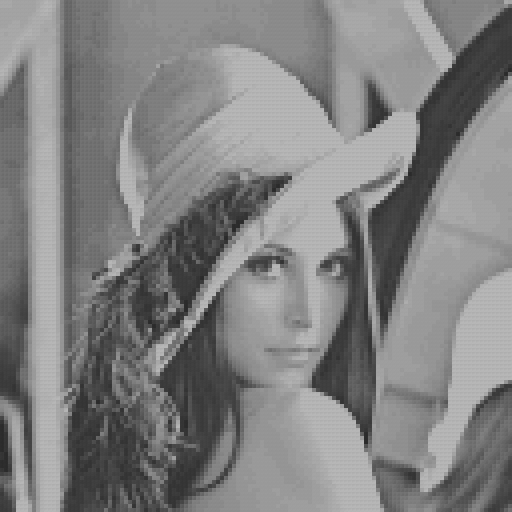
\includegraphics[width=10cm]{CB_neurons=40_block_size=4x4_50.png}
 \vspace{-0.3cm}
 \caption{Skompresowany obraz otrzymany z przypadku 1}
 \vspace*{\floatsep}

 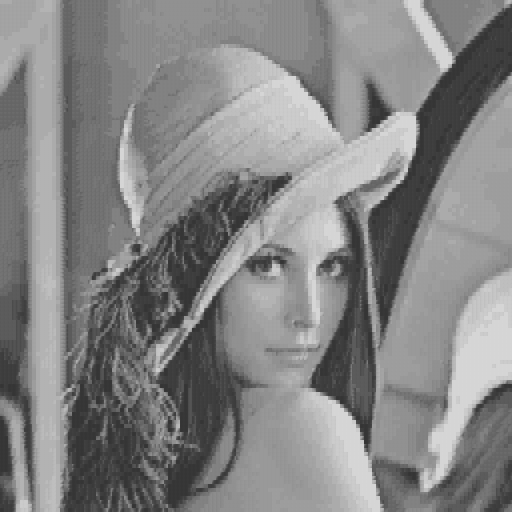
\includegraphics[width=10cm]{CB_neurons=40_block_size=4x4_50000.png}
 \vspace{-0.3cm}
 \caption{Skompresowany obraz otrzymany z przypadku 4}

\end{figure}
\clearpage

%%%%%%%%%%%%%%%%%%%%%%%%%%%%%%%%%%%%%%%%%%%%%%%%%%%%%%%%%%%%%%%%%%%%%%%%%%%%%%%%%%%%%%%%%%%%%%%%%%%%%%%%%%%%%%%%%
% PODROZDZIA£ PT. EKSPERYMENT NR 4
%%%%%%%%%%%%%%%%%%%%%%%%%%%%%%%%%%%%%%%%%%%%%%%%%%%%%%%%%%%%%%%%%%%%%%%%%%%%%%%%%%%%%%%%%%%%%%%%%%%%%%%%%%%%%%%%%

\subsection{Eksperyment nr 4}

Eksperyment nr 4 polegał sprawdzeniu jaki wpływ na kompresje obrazu ma krok uczący. Zrealizowane zostały 3 przypadki testowe przedstawione w Tab.  
\ref{dane eksperymentalne doświadczenia 4}. \\
\begin{table}[h!]
 \caption{Dane eksperymentalne nr 4}
 \centering
 \vspace{0.2cm}
 \begin{tabular}{c c}
  \hline\hline\\[-0.4cm]
  \textbf{Przypadek} & \textbf{Krok uczący} \\[0.1cm]
  \textbf{1} & 0.2  \\
  \textbf{2} & 0.5  \\
  \textbf{3} & 0.9  \\  [0.1cm]
  \hline
 \end{tabular}
 \label{dane eksperymentalne doświadczenia 4}
\end{table} \\

Dodatkowo, dla każdego z wyżej wymienionych przypadków ustawiliśmy następujące wartości: \\
\begin{table}[h!]
 \caption{Dodatkowe dane do eksperymentu nr 4}
 \centering
 \vspace{0.2cm}
 \begin{tabular}{c c c}
  \hline\hline\\[-0.4cm]
  \textbf{Ilość neuronów} & \textbf{Rozmiar ramki} & \textbf{Ilość ramek treningowych} \\[0.1cm]
  40 & 4x4 & 5000  \\ [0.1cm]
  \hline
 \end{tabular}
 \label{dodatkowe dane do eksperymentu nr 4}
\end{table} \\

\newpage
\subsubsection{Rezultat}

Wyniki powyższego doświadczenia przedstawiony został w Tab. 
\ref{wynik eksperymentu 4}.

\begin{table}[h!]
 \caption{Wynik eksperymentu nr 4}
 \centering
 \vspace{0.2cm}
 \begin{tabular}{c c c c}
  \hline\hline\\[-0.4cm]
  \textbf{Przypadek} & \textbf{MSR} & \textbf{PSNR} & \textbf{Compression Ratio} \\[0.1cm]
  \textbf{1} & 119.41 & 27.36 & 7.22  \\
  \textbf{2} & 122.68 & 27.24 & 6.89  \\
  \textbf{3} & 129.09 & 27.02 & 7.49  \\ [0.1cm]
  \hline
 \end{tabular}
 \label{wynik eksperymentu 4}
\end{table}

Eksperyment ten pokazał iż krok uczący nie ma dużego wpływu na jakość oraz stopień skompresowania obrazu. Im mniejszy krok uczący tym tym lepsza jakość wynikowego obrazu. Zdjęcia są na tyle podobne, iż zdecydowaliśmy się nie umieszczać przykładów w tym eksperymencie.


%%%%%%%%%%%%%%%%%%%%%%%%%%%%%%%%%%%%%%%%%%%%%%%%%%%%%%%%%%%%%%%%%%%%%%%%%%%%%%%%%%%%%%%%%%%%%%%%%%%%%%%%%%%%%%%%%
% PODROZDZIA£ PT. WNIOSKI
%%%%%%%%%%%%%%%%%%%%%%%%%%%%%%%%%%%%%%%%%%%%%%%%%%%%%%%%%%%%%%%%%%%%%%%%%%%%%%%%%%%%%%%%%%%%%%%%%%%%%%%%%%%%%%%%%
\newpage
\section{Wnioski}

Przeprowadzone eksperymenty pozwoliły nam zauważyć jak wartości badanych przez nas parametrów wpływają na stopień kompresji obrazu oraz jego jakość. \par
Eksperyment nr 1 pokazał nam jak duży wpływ ma ilość neuronów wyjściowych na stopień kompresji obrazu. Im więcej neuronów, tym mniejszy stopień kompresji, aczkolwiek znacząco poprawia się jakość skompresowanego obrazu. Należy też zwrócić uwagę, iż ilość neuronów wpływa też na czas, jaki potrzebny jest do wykonania kompresji, odpowiednio większa ilość neuronów zwiększa czas przetwarzania.\par
Eksperyment nr 2 polegał na sprawdzeniu wpływu wielkości ramki na poziom i jakość kompresji. Im większa ramka, tym lepszy poziom kompresji natomiast znacząco tracimy na jakości skompresowanego obrazu. Widzimy że w przypadku ramki 4x4 MSR wynosi 120, natomiast przy ramce 16x16 wynik ten jest prawie 3-krotnie większy. Różnice w stopniu kompresji nie są aż tak duże jak np. w eksperymencie 1.\par
Eksperyment nr 3 polegał na zmianie ilości ramek treningowych podawanych podczas treningu sieci. Tak jak się spodziewaliśmy, wraz ze wzrostem ilości ramek treningowych skompresowany obraz stawał się coraz bardziej dokładny. Ciekawym zjawiskiem był fakt, iż w przypadkach 1-3 wraz ze wzrostem ramek malał stopień kompresji, natomiast w przypadku 4, gdzie zastosowaliśmy największą ilość ramek treningowych, poziom kompresji okazał się większy niż w przypadku 2 i 3. Dzięki temu eksperymentowi możemy wywnioskować, że im większa ilość ramek treningowych tym lepszej jakości obraz otrzymamy oraz zostanie on lepiej skompresowany, ponieważ sam trening będzie dokładniejszy.\par
W eksperymencie nr 4 sprawdzaliśmy jaki wpływ miał krok uczący na kompresje obrazu. Rezultaty tego eksperymentu nie były dla nas zaskoczeniem, które potwierdziły fakt, że mniejszy krok uczący potrafi wytrenować sieć, która skompresuje lepszej jakości obraz. Różnica stopi kompresji między 1 i 3 przypadkiem jest niewielka, natomiast jakość kompresji w 1 przypadku jest już dużo lepsza.\par
Podsumowując, możemy zauważyć iż największą rolę w przypadku kompresji obrazu ma ilość neuronów, jaką podamy na wyjściu sieci neuronowej oraz wielkość ramki na jaki zostanie kompresowany obraz podzielony. Im większa ilość neuronów tym lepszej jakości obraz osiągniemy, natomiast sam obraz zostanie w mniejszym stopniu skompresowany. W przypadku wielkości ramki, im jest ona mniejsza, tym dokładniejsze odwzorowanie oryginalnego obrazu oraz mniejszy stopień kompresji. Ilość ramek treningowych oraz krok treningowy wpływa w głównej mierze na jakość obrazu końcowego, natomiast nie ma większego wpływu na stopień kompresji. Należy zwrócić uwagę, iż nie można jednoznacznie stwierdzić idealnych wartości wejściowych. Wszystko zależy od tego, czy zależy nam bardziej na lepszej jakości obrazu czy jak najmniejszym jego rozmiarze.


%%%%%%%%%%%%%%%%%%%%%%%%%%%%%%%%%%%%%%%%%%%%%%%%%%%%%%%%%%%%%%%%%%%%%%%%%%%%%%%%%%%%%%%%%%%%%%%%%%%%%%%%%%%%%%%%%
% BIBLIOGRAFIA
%%%%%%%%%%%%%%%%%%%%%%%%%%%%%%%%%%%%%%%%%%%%%%%%%%%%%%%%%%%%%%%%%%%%%%%%%%%%%%%%%%%%%%%%%%%%%%%%%%%%%%%%%%%%%%%%%

\renewcommand\refname{Bibliografia}
\bibliographystyle{plain}
\begin{thebibliography}{0}
\bibitem{l2short} T. Oetiker, H. Partl, I. Hyna, E. Schlegl.
\textsl{Nie za krótkie wprowadzenie do systemu \LaTeX2e}, 2007, dostępny online.
\bibitem{12short} T. Kohonen.
\textsl{Self-organising Maps. Springer, Berlin - Heidelberg}1995.
\bibitem{12short} E. Skubalska-Rafajłowicz, M. Nałęcz.
\textsl{Samo-organizujące sieci neuronowe. Biocybernetyka i Inżynieria Biomedyczna }2000, Tom 6: Sieci neuronowe, str. 187–188
\bibitem{12short}M. Krętowska
\textsl{Katedra Oprogramowania, Wykład 11: Sieci samo organizujące się} 2011, Białystok, Katedra Oprogramowania.
\end{thebibliography}

\end{document}
